\documentclass[%
 reprint,
%superscriptaddress,
%groupedaddress,
%unsortedaddress,
%runinaddress,
%frontmatterverbose, 
%preprint,
%showpacs,preprintnumbers,
%nofootinbib,
%nobibnotes,
%bibnotes,
 amsmath,amssymb,
 aps,
 pra,
%prb,
%rmp,
%prstab,
%prstper,
%floatfix,
]{revtex4-1}

\usepackage{graphicx}% Include figure files
\usepackage{dcolumn}% Align table columns on decimal point
%\usepackage{bm}% bold math
\usepackage{fullpage}
\usepackage{epsfig}
\usepackage{amsmath}
\usepackage{amsfonts}
\usepackage{amssymb}
\usepackage{float}
\usepackage{pstricks}
\usepackage{cancel}
\usepackage{lipsum}
%\usepackage[nottoc,numbib]{tocbibind} %Uncomment for bibliography to be its own numbered section
\usepackage{units}
\usepackage{listings}

\graphicspath{{./plots/}}

\begin{document}

\preprint{APS/123-QED}

\title{\textbf{Lab Report: X-Ray Diffraction and Florescence} \\ \small{An Investigation of Characteristic Transitions of Atoms}}
\author{Joshua LaBounty}
\author{Thomas Krahulik}
\affiliation{Stony Brook University --- PHY 445}

\date{\today}

\begin{abstract}
	In this experiment, we investigate the characteristic x-rays produced by atomic transitions of various elements, according to Moseley's Law. 
\end{abstract}
\maketitle

\section{Introduction}

\section{Review of Previous Work}

\section{Experimental Setup}

\subsection{X-Ray Florescence}

\begin{figure}[H]
	\centering
	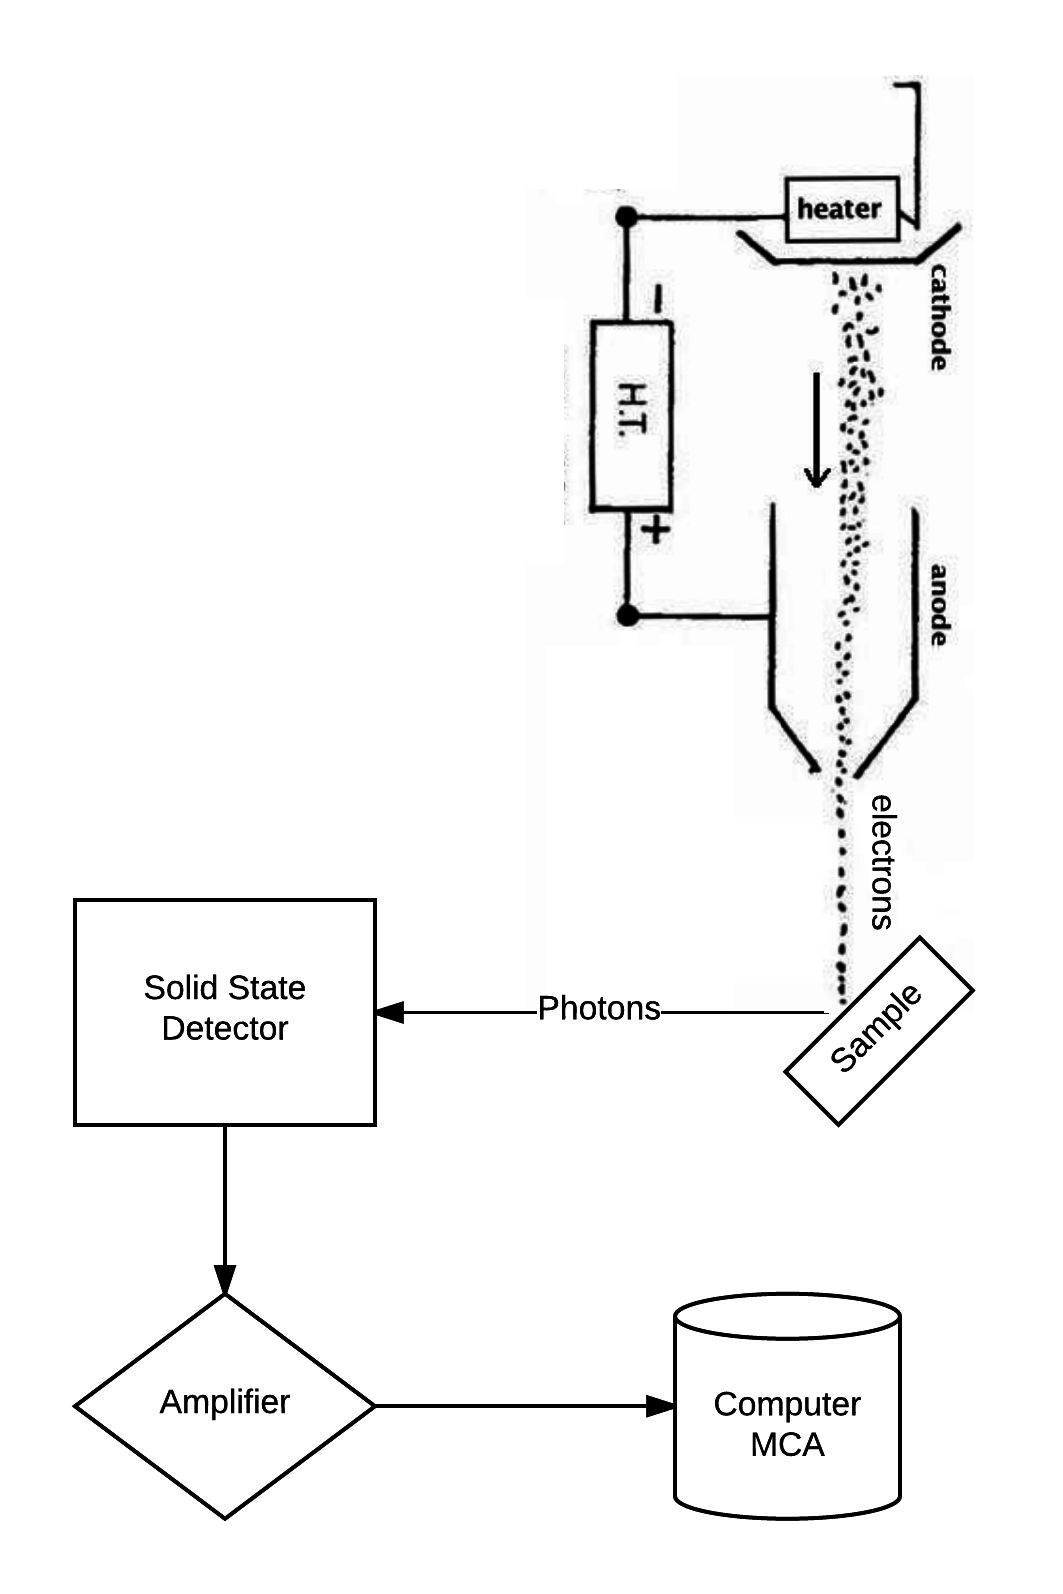
\includegraphics[width=0.25\textwidth]{xrf_experiment.png}
	\caption{Experimental Setup used in XRF portion of the experiment.}
	\label{fig:xrf_setup}
\end{figure}

The apparatus used in our measurements of x-ray florescence consists primarily of two components, an electron gun and a solid state detector, as shown in Figure \ref{fig:xrf_setup}. The electron gun operates by running a current through a filament, typically made out of tungsten due to its resilience to high temperatures, in a potential. Electrons are 'boiled off' the filament (a process known as thermionic emission) and are accelerated towards the anode. Some of the electrons strike the anode, but the rest escape through the opening into a collimated beam of particles. The energy of these electrons is defined by their accelerating voltage: $E_{e^-} = qV$, while their number is defined by the current.  These electrons impact the sample and cause it to emit photons, which are then picked up by the detector. The detector is a Silicon p-i-n diode manufactured by Amptek. Photons which are incident on the detector are first met with a window made of Beryllium, which is opaque to photons whose energies are below $\approx ~1~keV$. Photons whose energies are high enough to pass through this window then deposit their energy in the sensitive volume of the detector, ionizing the silicon atoms and creating a number of electron-hole pairs in the lattice structure. A bias voltage across the diode causes these electron/holes to flow and be read into the detector as a pulse of charge, whose magnitude is directly proportional to the energy which was deposited in the detector by the photons. This pulse is passed through an amplifier, which is then passed into the multi-channel analyzer (MCA), and then from there into the computer system. From there, the information is saved in a format which can be read into our data analysis software, ROOT. This software is developed and maintained by scientists at CERN, and contains many useful fitting and histogram manipulation packages. We also performed independent cross checks of its $\chi^2$ minimization techniques, which can be found in Appendix \ref{section:root}.

\subsection{X-Ray Diffraction}

\begin{figure}[H]
	\centering
	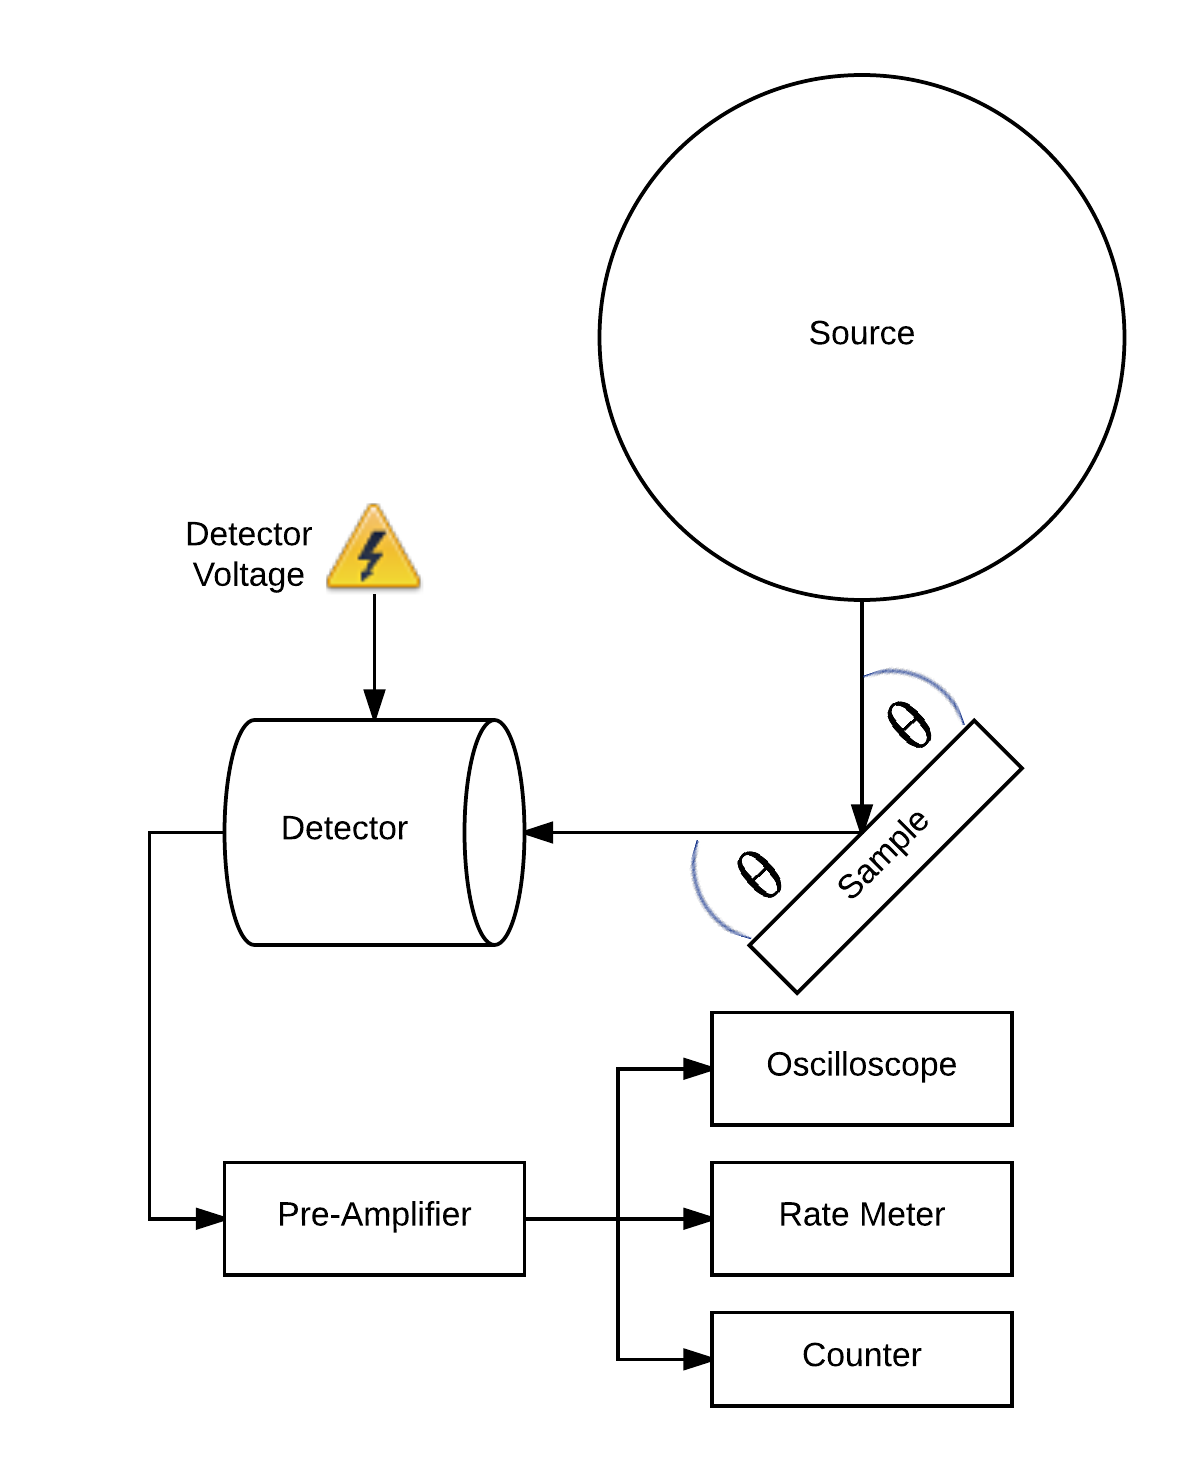
\includegraphics[width=0.3\textwidth]{xrd_experiment.png}
	\caption{Experimental Setup used in XRD portion of the experiment.}
	\label{fig:xrd_setup}
\end{figure}

This experiment consists of three primary components, the 

\section{Measurements}

\subsection{X-Ray Florescence}

Before performing an analysis of x-ray fluorescence, we had to calibrate the energy scale of the MCA to determine the conversion between the channel number ($n$) of a detected photon and its energy. In order to perform this calibration, x-ray fluorescence spectra were collected for various samples with known energy peaks. Fig.~\ref{} displays an example spectrum with fitted peaks.

\begin{figure}[H]
	\centering
	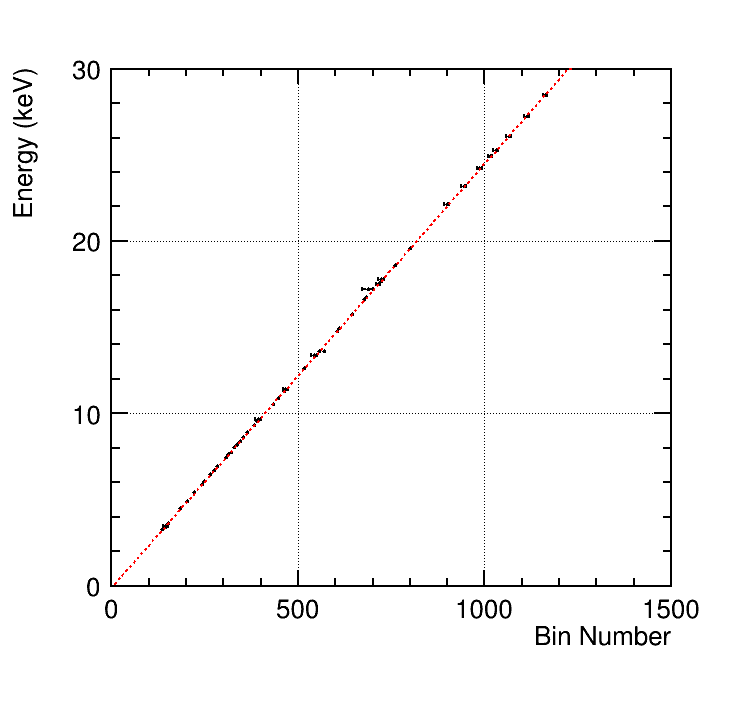
\includegraphics[width=0.45\textwidth]{EvsBin.png}
	\caption{Energy vs Channel Number Calibration Plot}
	\label{Fig:Evsbin}
\end{figure}

Each peak on one of these spectra was fit with a Gaussian distribution to find the mean value of the peak. This mean value was stored as the bin number corresponding to the peak of known energy provided by external sources. We collected corresponding energies and bin numbers for several samples of different elements to generate the energy vs bin number plot in Fig.~\ref{Fig:Evsbin}.

\begin{figure}[H]
	\centering
	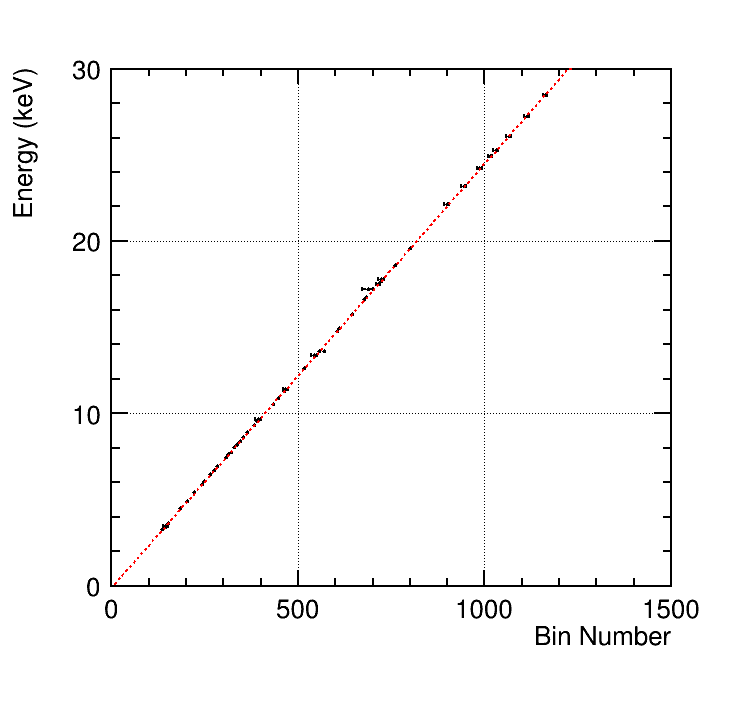
\includegraphics[width=0.45\textwidth]{EvsBin.png}
	\caption{Energy vs Channel Number Calibration Plot}
	\label{Fig:Evsbin}
\end{figure}

The linear fit on this plot provided us with the energy calibration in Eq.~\ref{eq:ECalib}.
\begin{gather}\label{eq:ECalib}
E = 0.0245644n - 0.0545754
\end{gather}

With this calibration, we could then calculate the energies of peaks in our x-ray fluorescence spectra.



\begin{figure}[H]
	\centering
	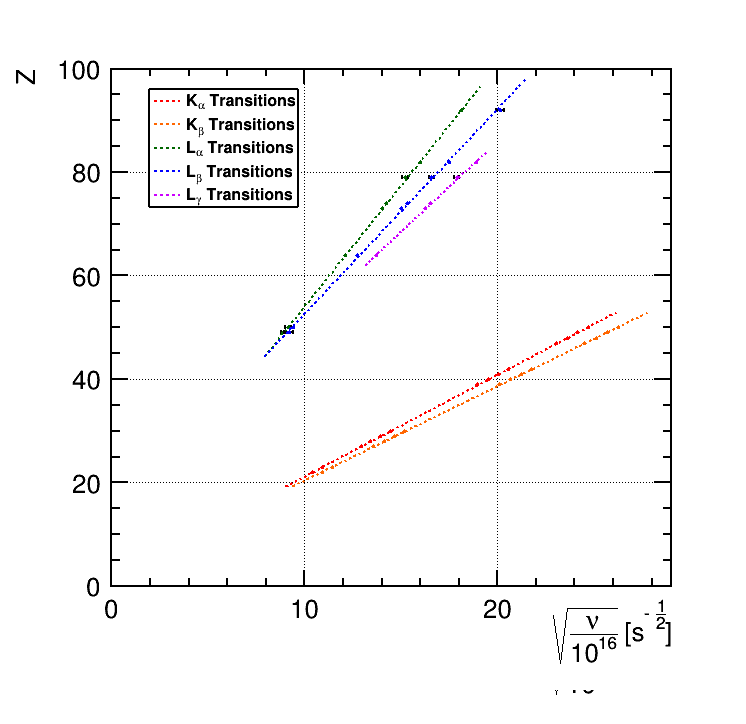
\includegraphics[width=0.48\textwidth]{MoseleyLawPlot.png}
	\caption{Plot Displaying Moseley's Law for $K_{\alpha}$, $K_{\beta}$, $L_{\alpha}$, $L_{\beta}$, and $L_{\gamma}$ Transitions}
	\label{Fig:Evsbin}
\end{figure} 

\subsection{X-Ray Diffraction}

\subsubsection{Characterization of the Detector}

\section{Theoretical Model}

\subsection{X-Ray Florescence}

\subsection{X-Ray Diffraction}

\section{Comparison of Theory and Experiment}

\subsection{X-Ray Florescence}

\subsection{X-Ray Diffraction}

\section{Discussion}

\section{Author Contributions}

\begin{thebibliography}{6}
	
	\bibitem{milissinos}
	A.C. Melissinos, Experiments in Modern Physics (Academic Press, NY, 1966).
	
	\bibitem{bevington}
	Philip R. Bevington and D. Keith Robinson, Data Reduction and Error Analysis 3rd edition (McGraw-Hill, 2003).
	
	\bibitem{eisberg}
	R. M. Eisberg et al., Chapter 14: X-Rays. Fundamentals of Modern Physics,  (Wiley, 1961), Physics Library Ref. QC173.E38.

	\bibitem{frenchtable}
	Laboratoire National Henri Becquerel. Table de Radionucléides (2015) \url{http://www.nucleide.org/DDEP_WG/Nuclides/Cs-137_tables.pdf}
	
	\bibitem{xrd_report}
	Mihaly, Laszlo and PMK. X-Ray Diffraction. (Stony Brook University, 2001)


\end{thebibliography}

\begin{appendix}

\section{Validation of the $\chi^2$ Minimization in ROOT} \label{section:root}
For this experiment, we used ROOT, a c++ based data analysis software, to plot and fit functions to our data. To verify that ROOT calculates a correct value for $\chi^{2}$, we performed a hand calculation cross check with a simple set of data. The data set we used for this cross check was $\{ (11.0 \pm 0.0, 23.0 \pm 0.5), (14.0 \pm 0.0, 25.0 \pm 0.5), (20.0 \pm 0.0, 35.0 \pm 0.5), (25.0 \pm 0.0, 39.0 \pm 0.5) \}$. We plotted this data and fit it to a linear function $f(x) = [0] + [1]*x$. This plot is shown in Fig.~\ref{Fig:rootproof}.
\begin{figure}[H]
	\centering
	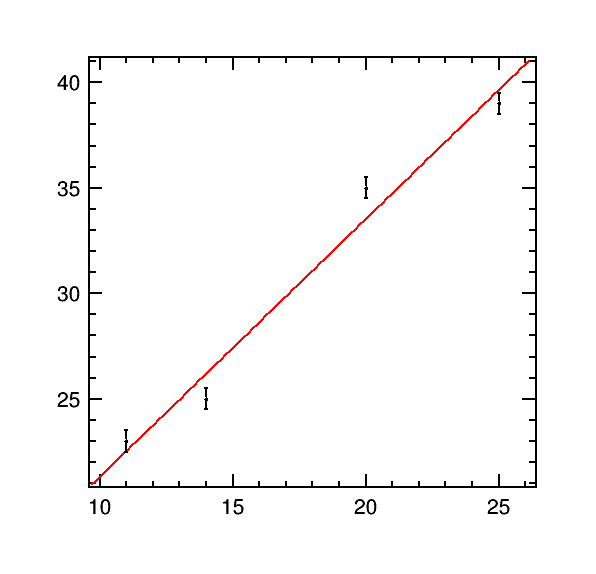
\includegraphics[width=0.4\textwidth]{rootproof.png}
	\caption{Sample Data Fitted to a Line}
	\label{Fig:rootproof}
\end{figure}
The function obtained from this fit was $f(x) = 9.11111 + 1.22222x$ with a chi-squared of $\chi ^{2} = 16.8889$. We then performed a hand calculation of the $\chi ^{2}$ using Eq.~\ref{eq:chisq}.
\begin{gather}\label{eq:chisq}
\chi ^{2} = \sum \frac{(f(x_i) - y_i)^{2}}{\sigma_i^2}
\end{gather}
When performing this hand calculation we also obtained a value of $\chi ^{2} = 16.8889$, verifying ROOT's ability to calculate $\chi ^{2}$.
\begin{align*}
\chi ^{2} =& \frac{(f(11.0) - 23.0)^{2}}{(0.5)^2} + \frac{(f(14.0) - 25.0)^{2}}{(0.5)^2} \\
&+ \frac{(f(20.0) - 35.0)^2}{(0.5)^2} + \frac{(f(25.0) - 39.0)^{2}}{(0.5)^2} \\
&= 16.8889
\end{align*}

\section{Analysis Code} \label{section:analysis_code}
All of the analysis code used for this lab can be found in the following git repository: 
\begin{verbatim}
https://github.com/jlabounty/SeniorLab/tree
/master/XRF_XRD
\end{verbatim}

\end{appendix}

\end{document}